\documentclass[12pt]{article}
\usepackage[utf8]{inputenc}
\usepackage{graphicx}
\graphicspath{ {./images/} } % Uncomment
\usepackage[
top=2cm,
bottom=2cm,
left=2cm,
right=2cm,
headheight=17pt, % as per the warning by fancyhdr
includehead,includefoot,
heightrounded, % to avoid spurious underfull messages
]{geometry} 
\geometry{a4paper}
\usepackage{fancyhdr}

% Lecture Name, exercise number, group number/members
\newcommand{\lecture}{GPU Computing}
\newcommand{\exercise}{Exercise 4}
\newcommand{\groupnumber}{gpucomp03}
\newcommand{\groupmembersshort}{Benjamin Maier, Daniel Barley, Laura Nell}
\newcommand{\groupmemberslist}{Benjamin Maier\\Daniel Barley\\Laura Nell}
\newcommand{\duedate}{December 1st, 09:00}



\fancyhf{}
\fancyhead[L]{\groupnumber}
\fancyhead[R]{\textsc{\groupmembersshort}}
\fancyfoot[C]{\lecture: \exercise}
\fancyfoot[R] {\thepage}
\renewcommand{\headrulewidth}{0.4pt}
\renewcommand{\footrulewidth}{0.4pt}
\pagestyle{fancy}

\begin{document}
	\begin{titlepage}
		\centering

		{\scshape\LARGE Heidelberg University\\Institute for Computer Engineering (ZITI) \par}
		\vspace{1.5cm}
		{\scshape\Large Master of Science Computer Engineering \par}
		\vspace{0.5cm}
		{\scshape\Large \lecture \par}
		\vspace{1.5cm}
		{\huge\bfseries \exercise \par}
		\vspace{2cm}
		{\Large \groupnumber \itshape \\ \vspace{30pt} \groupmemberslist \par}
		\vfill
		
		
		% Bottom of the page
		{\large Due date \duedate \par}
	\end{titlepage}

\setcounter{section}{4}

\subsection{Reading}
\subsubsection*{Debunking the 100X GPU vs. CPU myth: an evaluation of throughput computing on CPU and GPU}
Because of the massive amount of generated data, it is important for throughput computing applications that handle with these data to have a reasonable amount of data prallelism. Such applications can be realized for CPUs or GPUs. Because of their different architectures, they perform different for different throughput computing workloads and have different possibilities for optimizations. Thus, 14 throughput computing kernels with different characteristics are compared based on their execution on the Intel Core i7 CPU and the Nvidia GTX280 GPU.\\\\
The performance of the several kernels depends highly on their requirements and the corresponding architecture of the devices like bandwidth limitations, compute flops, cache size or synchronization.\\
Typically the highest performance is achieved when a suitable number of multiple threads are used per core.\\
Nevertheless, the performance gap between CPU and GPU can be a lot decreased (down to an average of 2.5X) by indvidual optmizations of software and hardware on both devices. Main optimizations for CPUs leading to performance improvements are multithreading, cache blocking and reorganization of memory accesses for SIMDfication. Optimizations that lead to GPU performance improvements are minimizing global synchronization and using local shared buffers.\\
Besides that, the key hardware architecture features which lead to an imporved performance are identified.\\\\
The main characteristics of performance differences still fit for todays architectures, while the overall performance and functionality of CPUs and GPUs has actually improved. Thus, we accept the paper and its content.

\vspace{10pt}


\subsubsection*{NVIDIA Tesla: A Unified Graphics and Computing Architecture}

To enable flexible, programmable graphics and high-performance computing, NVIDIA has developed the Tesla scalable unified graphics and parallel computing architecture, which extends the functionality of traditional graphics pipelines. The goal for that architeture was to unify vertex and pixel processors in one architecture.\\
The developed architecture itself along with the resulting (parallel) workflows is described before an overview of the parallel programming model in C with CUDA tools is given.\\\\
There are many innovations in the Tesla architecture, including the execution of scalar instructions or the SIMT processor architecture, which enables executing threads grouped into several warps and increases the efficiency a lot.\\
Regarding the programming model, the Tesla architecture introduces cooperative thread arrays or CUDA thread blocks to ensure the correct execution of a large number of concurrent threads.\\
The Tesla architecture was developed for scalability also with large problem sizes. Thus, GPUs using this architecture deliver high performance also for demanding parallel-computing and graphics applications. \\\\
Nvidia was one major driver in the development of GPUs and corresponding architectures as highly parallel general purpose computers. Thus, also the Tesla architecture had, at this time, some great new improvements for graphics processing and lead to further innovations. We therefore fully accept the paper and its content.
\vspace{10pt}

\subsection{Shared Memory Analysis - Basis}

\begin{figure}
	\centering
	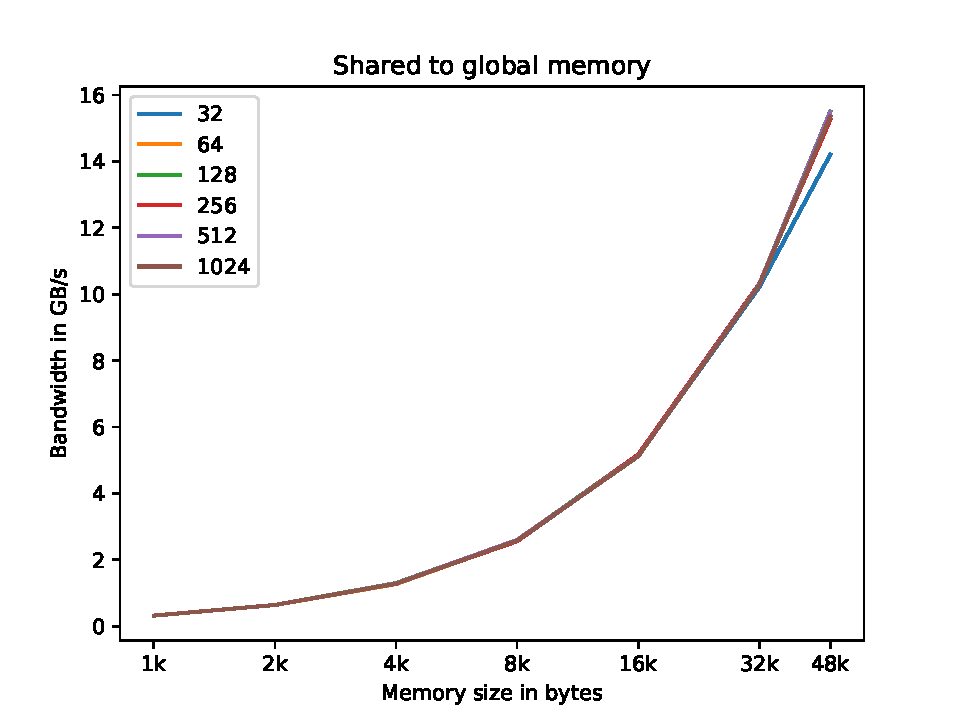
\includegraphics[width=0.7\linewidth]{../../template/plots/aufgabe4_2a}
	\caption{Global to shared memory}
	\label{fig:aufgabe42a}
\end{figure}

\begin{figure}
	\centering
	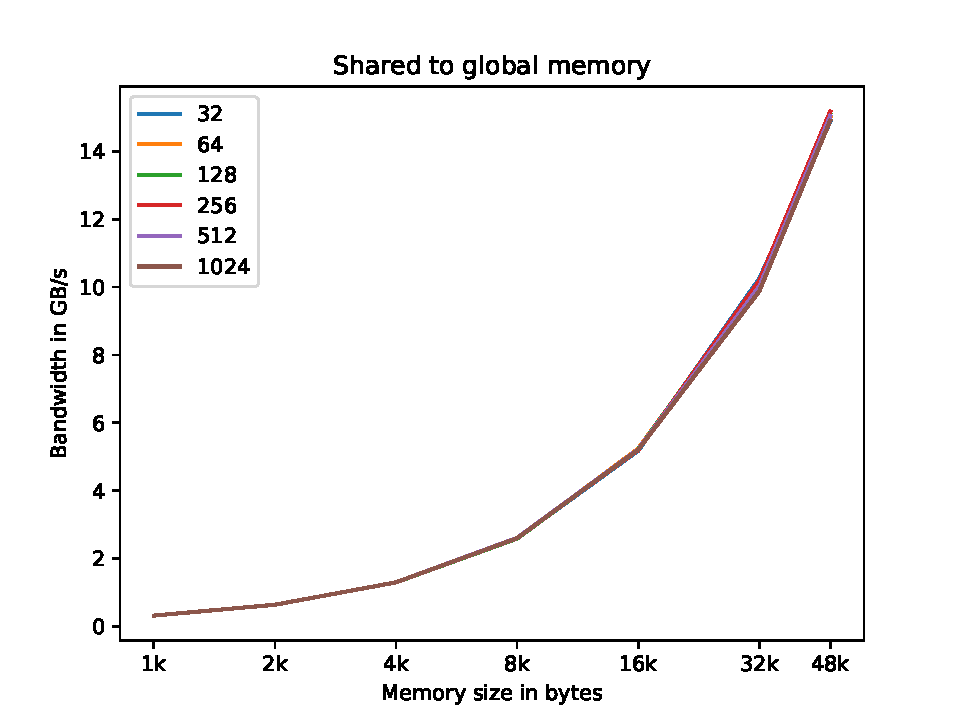
\includegraphics[width=0.7\linewidth]{../../template/plots/aufgabe4_2b}
	\caption{Shared to global memory}
	\label{fig:aufgabe42b}
\end{figure}

For the basic versions (figure \ref{fig:aufgabe42a} and \ref{fig:aufgabe42b}) we could not find any influence of the amount of threads. However, we decided to start with a thread amount of 32, since below we would not fully utilize the gpu.

\begin{figure}
	\centering
	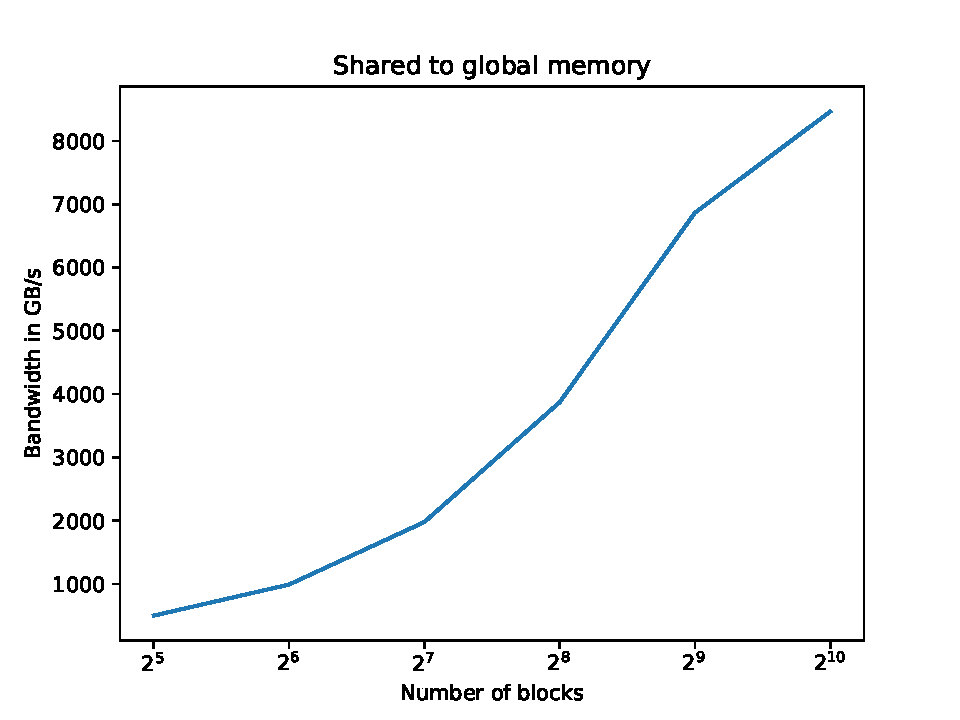
\includegraphics[width=0.7\linewidth]{../../template/plots/aufgabe4_2c}
	\caption{Global to shared memory}
	\label{fig:aufgabe42c}
\end{figure}

\begin{figure}
	\centering
	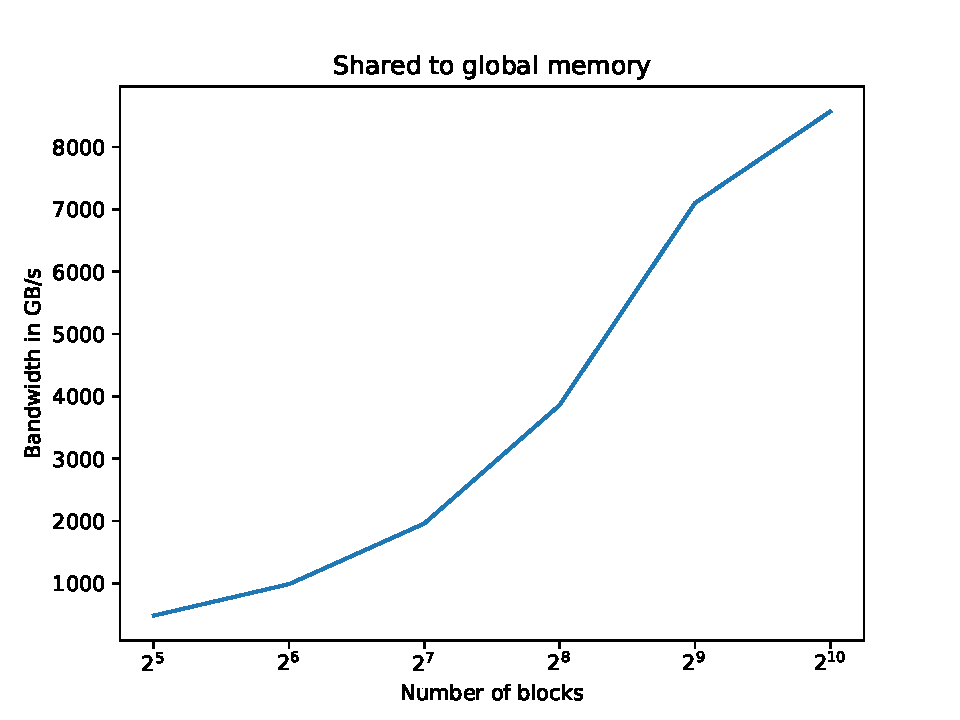
\includegraphics[width=0.7\linewidth]{../../template/plots/aufgabe4_2d}
	\caption{Shared to global memory}
	\label{fig:aufgabe42d}
\end{figure}

For the next task we should vary the number of blocks. In figure \ref{fig:aufgabe42c} and \ref{fig:aufgabe42d} one can see that the throughput scales linear with the amount of blocks. The reason for this is that every block has its own amount of shared memory and so the throughput gets added.

\begin{figure}
	\centering
	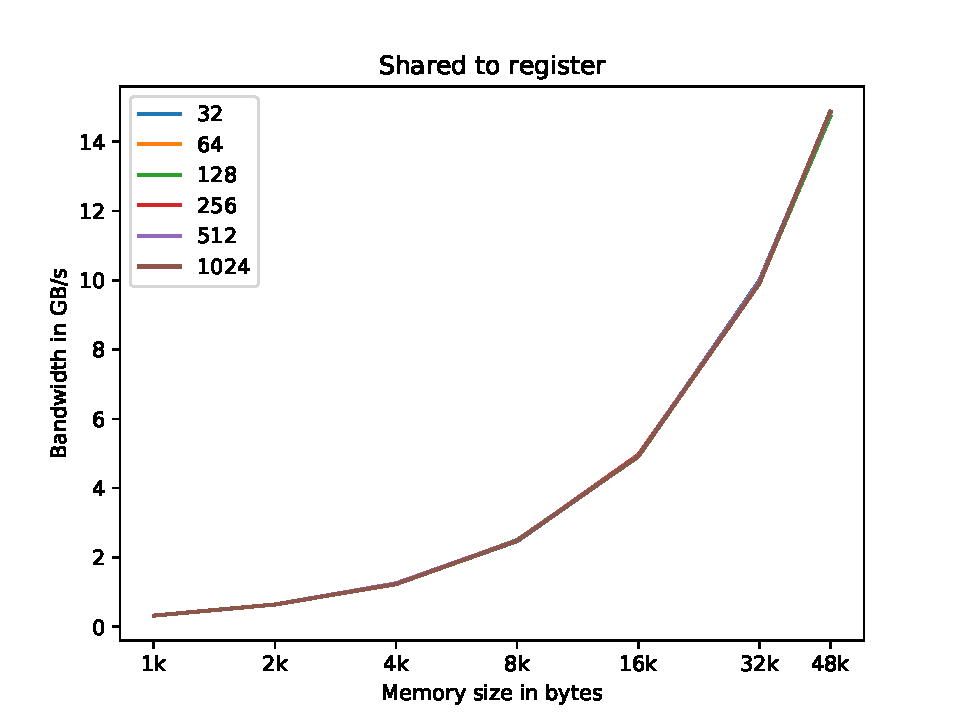
\includegraphics[width=0.7\linewidth]{../../template/plots/aufgabe4_2e}
	\caption{Global to shared memory}
	\label{fig:aufgabe42e}
\end{figure}

\begin{figure}
	\centering
	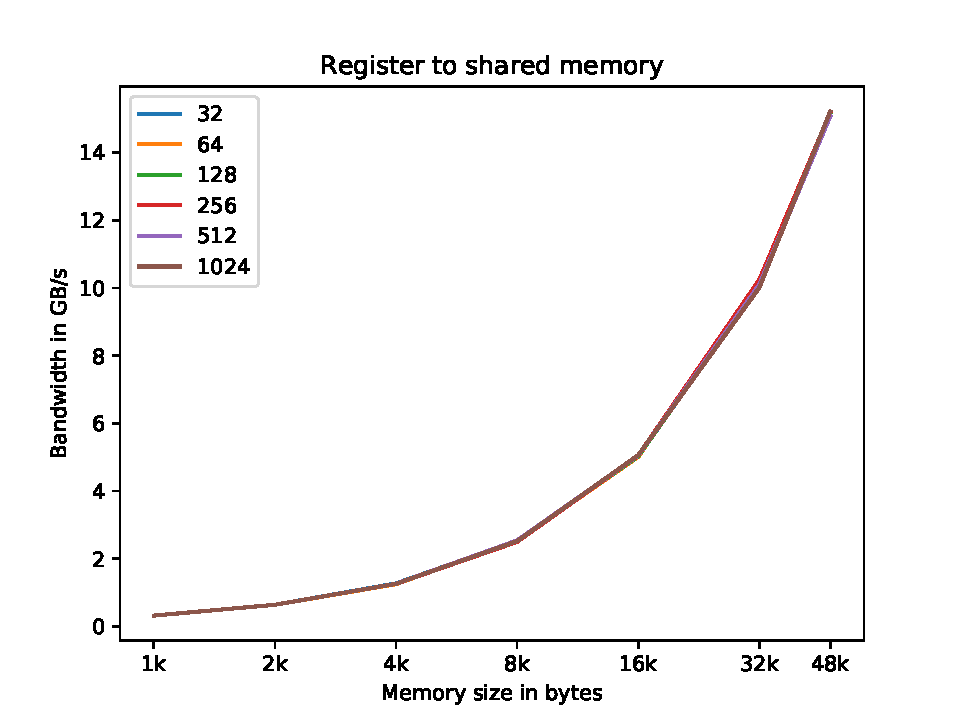
\includegraphics[width=0.7\linewidth]{../../template/plots/aufgabe4_2f}
	\caption{Shared to global memory}
	\label{fig:aufgabe42f}
\end{figure}

Finally we should meassure a simple shared memory to register transfer. The results are shown in figure \ref{fig:aufgabe42e} and \ref{fig:aufgabe42f}. Again we cannot see a big difference. \\

\begin{figure}
	\centering
	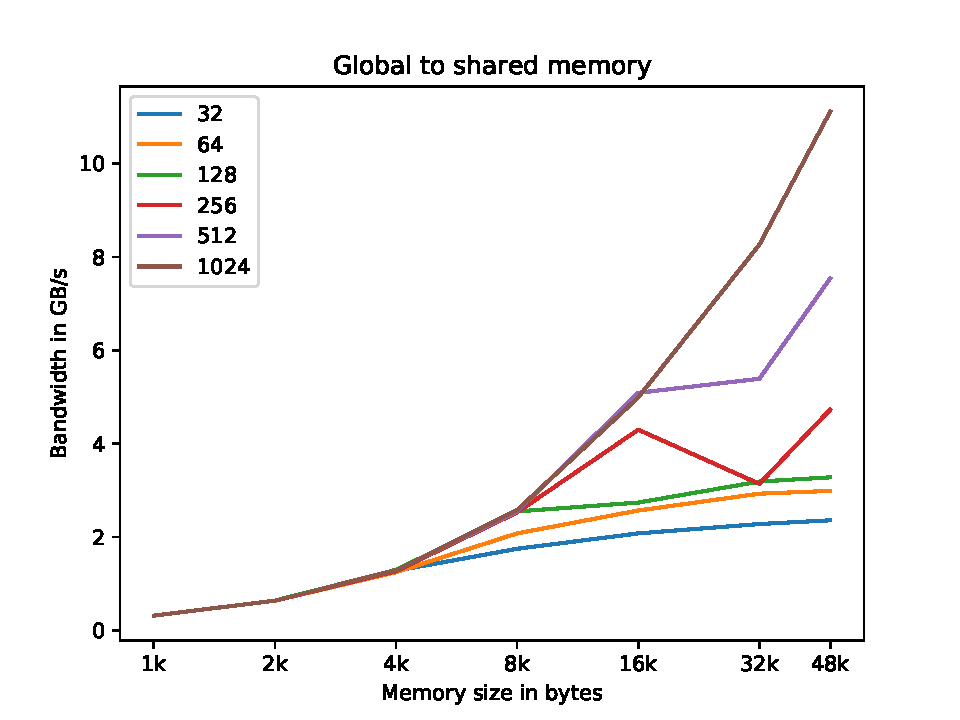
\includegraphics[width=0.7\linewidth]{../../template/plots/aufgabe4_2a_v2}
	\caption{Global to shared memory with consecutively access pattern.}
	\label{fig:aufgabe42av2}
\end{figure}


Here at this point we would like to add some remars according to the code. General spoken there are two main methods to access the data inside the kernel: (i) consecutively inside a thread, (ii) strided across the threads inside a block. The benefit of the second method is the better useage of the L1 cache. To verify this we repeated the first measurement with the first method. The results are shown in figure \ref{fig:aufgabe42av2}. According to the results we decided to use the second access pattern for the rest of the exercise. Maybe this is the reason why our meassurements show similar results. 




\subsection{Shared Memory Analysis - Conflicts}

\begin{figure}
	\centering
	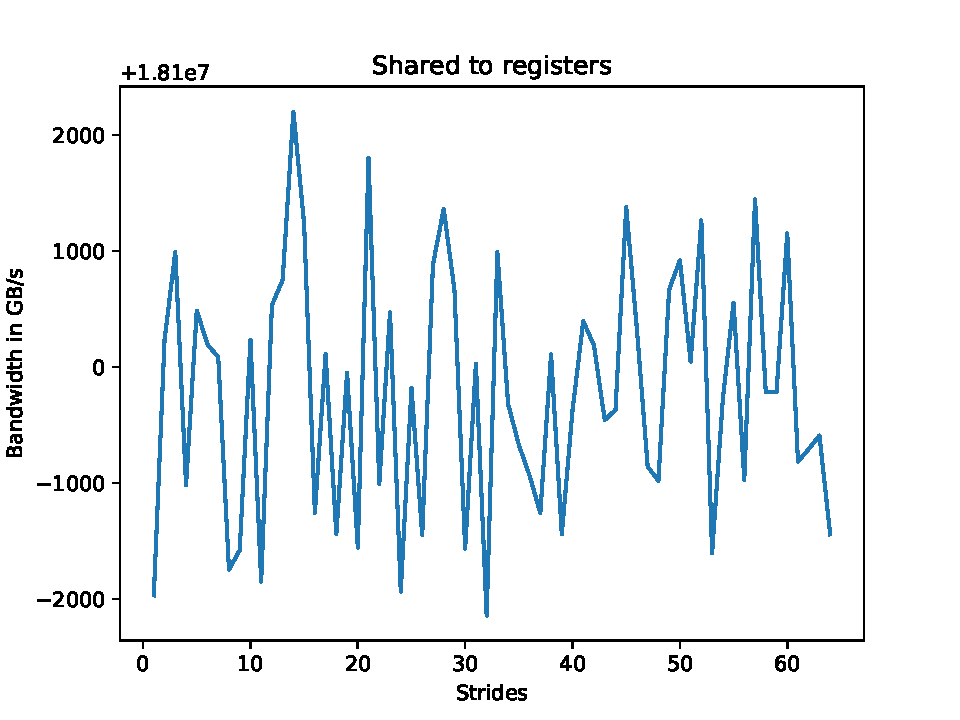
\includegraphics[width=0.7\linewidth]{../../template/plots/aufgabe4_3}
	\caption{Bank conflicts}
	\label{fig:aufgabe43}
\end{figure}

In the next exercise we should try to meassure the impact of bank conflicts. However, as you can see in figure \ref{fig:aufgabe43}, we cannot find a impact of the strided access pattern. Maybe there is a error in our code. Normally you would expect that with a multiple of the bank size, you get alot of conflicts and therefore have a higher clock count.


\subsection{Matrix Multiply - CPU Sequential Version}

\subsection{Willingness to present}
Hereby, we declare our will to present the results presented in the former sections.


\end{document}